\section{Experiments}

\subsection{Experimental Setup}
\subsubsection{Datasets}
We conduct experiments on 7 real-world datasets spanning various scales and domains: Reddit~\citep{RedWei}, Weibo~\citep{RedWei}, Amazon~\citep{Amazon}, YelpChi~\citep{YelpChi}, T-Finance~\citep{BWGNN}, Tolokers and Questions~\citep{TolQue}. 
We provide key dataset statistics in Table \ref{Tab: Dataset statistics}.
\begin{table}[t]
    \begin{center}
    % \setlength{\tabcolsep}{3.5pt}
     % \renewcommand\arraystretch{0.9}
    {\caption{Key details of seven evaluation datasets }\label{Tab: Dataset statistics}}
    \resizebox{\columnwidth}{!}{
    \begin{tabular}{lccccccc}
    \toprule
    \textbf{Dataset} & \#\textbf{Nodes} & \#\textbf{Edges} & \#\textbf{Feat.} & \#\textbf{Anomaly} & \#\textbf{Edge} \\
     & & & & \textbf{Nodes} & \textbf{Hetero.} \\
    \midrule 
    Amazon & 11,944 & 4,398,392 & 25 & 9.5\% & 0.046 \\
    YelpChi & 45,954 & 3,846,979 & 32 & 14.5\% & 0.227 \\
    T-Finance & 39,357 & 21,222,543 & 10 & 4.6\% & 0.029 \\
    Tolokers & 11,758 & 519,000 & 10 & 21.8\% & 0.405\\
    Reddit & 10,984 & 168,016 & 64 & 3.3\% & 0.053\\
    Weibo & 8,405 & 407,963 & 400 & 10.3\% & 0.023\\
    Questions & 48,921 & 153,540 & 301 & 3.0\% & 0.160\\
    \bottomrule
    \end{tabular}
    }
    \end{center}
\end{table}
\subsubsection{Baselines}
We compare our model with a series of baseline methods, which can be categorized into three groups.
The first group consists of methods based on standard GNNs, including GCN~\citep{GCN}, SAGE~\citep{SAGE}, and GAT~\citep{GAT}. 
The second group contains GNNs specifically designed for anomaly detection tasks, including PCGNN~\citep{PCGNN}, ConsisGAD~\citep{ConsisGAD}, and GAGA~\citep{GAGA}.
The third group comprises spectral GNN methods, namely
AMNet~\citep{AMNet}, BWGNN~\citep{BWGNN}, GHRN~\citep{GHRN}, ChiGAD~\citep{ChiGAD}, SEC-GFD~\citep{SEC-GFD}, DSGAD~\citep{DSGAD}.
% For detailed descriptions of these baselines, please kindly see Appendix \ref{App: Baselines}.
\subsubsection{Evaluation Metrics and Implementation Details}
% Following GADBench~\citep{GADBench}, we evaluate performance using the Area Under the Receiver Operating Characteristic Curve (AUROC), the Area Under the Precision-Recall Curve (AUPRC) calculated via average precision as metrics, with 100 labeled nodes (20 anomalies) per training set. 
% All experiments are averaged over 10 random splits provided by GADBench for robustness.
% \subsubsection{Model Hyperparameters and 
% Implementation Details.}
Following GADBench~\citep{GADBench}, we use AUROC and AUPRC metrics, with AUPRC computed as average precision. Each training split contains 100 labeled nodes, including 20 anomalies, and all results are averaged over the 10 random splits provided by GADBench to ensure robust evaluation.

The hyperparameters of the compared baselines are taken directly from the GADBench and/or the authors' implementations.  Hyperparameters of our proposed ESO-GAD are selected from predefined ranges, which are described in Appendix~\ref{app:details}.
Our code will be published upon acceptance.
\subsection{Main Results}\label{sec:experimental-results}
\label{sec:rq1}
\begin{table*}[t]
\centering
\caption{Results with mean $\pm$ std on seven real-world datasets in terms of AUROC.
The bold and underlined values denote the best and second-best results, respectively.}
\setlength{\tabcolsep}{5.5pt}
\renewcommand{\arraystretch}{1.08}

\resizebox{\textwidth}{!}{%
\begin{tabular}{lccccccc}
\toprule
\textbf{Methods}
& \textbf{Amazon}
& \textbf{YelpChi}
& \textbf{T-Finance}
& \textbf{Toloker}
& \textbf{Reddit}
& \textbf{Weibo }
& \textbf{Questions}\\
\midrule

% Group 1: General GNN baselines
GAT
& \val{92.44}{1.92}
& \val{65.26}{4.00}
& \val{84.98}{4.55}
& \val{68.06}{2.98}
& \val{60.55}{3.88}
& \val{86.83}{7.70} 
& \val{62.32}{1.46}\\

GCN
& \val{82.03}{0.33}
& \val{51.15}{3.70}
& \val{88.22}{2.36}
& \val{64.22}{4.82}
& \val{56.90}{5.93}
& \val{93.47}{6.58} 
& \val{59.99}{2.30}\\

GraphSAGE
& \val{79.23}{3.06}
& \val{59.79}{5.12}
& \val{69.24}{3.70}
& \val{67.40}{3.17}
& \val{58.59}{6.35}
& \val{81.00}{5.78} 
& \val{61.58}{2.90}\\

\midrule

% Group 2: Graph fraud detection baselines
PCGNN
& \second{93.22}{1.21}
& \val{65.09}{4.80}
& \val{92.01}{1.12}
& \val{67.38}{2.09}
& \val{52.83}{3.44}
& \val{83.90}{8.08}
& \val{59.03 }{4.21} \\

ConsisGAD
& \val{93.05}{1.41}
& \val{62.70}{4.44}
& \best{94.53}{1.25}
& \val{67.79}{2.48}
& \val{58.71}{3.82}
& \val{77.59}{2.52}
& \val{61.92 }{6.12}\\

GAGA
& \val{91.11}{2.12}
& \val{53.48}{4.26}
& \val{86.64}{10.42}
& \val{60.52}{4.24}
& \val{56.79}{2.72}
& \val{71.23}{11.98}
& \val{51.29}{2.78}\\

\midrule

% Group 3: Main comparison methods
BWGNN
& \val{91.90}{2.16}
& \val{64.39}{3.36}
& \val{92.12}{2.75}
& \val{68.42}{2.72}
& \val{57.72}{4.96}
& \val{93.65}{3.99}
& \val{60.18}{5.02}\\

ChiGNN
& \val{92.58}{2.23}
& \val{63.64}{3.83}
& \val{91.99}{1.00}
& \val{67.50}{5.64}
& \val{58.82}{4.58}
& \val{83.58}{3.98}
& \val{60.46}{6.98}\\

GHRN
& \val{90.99}{1.98}
& \val{63.45}{3.43}
& \val{92.58}{0.65}
& \second{69.01}{2.18}
& \val{57.53}{4.53}
& \val{91.62}{4.41} 
& \val{60.54}{7.11}\\

AMNet
& \val{92.74}{2.13}
& \val{64.80}{5.24}
& \val{92.66}{0.85}
& \val{61.62}{4.01}
& \second{62.95}{1.79}
& \val{82.39}{4.57}
& \second{63.59}{3.07}\\

SEC-GFD
& \val{91.23}{2.35}
& \second{65.27}{2.69}
& \val{90.92}{1.89}
& \val{67.80}{3.39}
& \val{57.04}{3.37}
& \val{93.90}{3.94}
& \val{62.03}{3.14}\\

DSGAD
& \val{92.07}{2.21}
& \val{62.93}{2.54}
& \val{93.22}{1.16}
& \val{66.35}{2.75}
& \val{59.39}{5.73}
& \second{94.11}{1.23}
& \val{60.09}{6.23}\\

\midrule

% Group 4: Proposed method
\textbf{ESO-GAD (ours)}
& \best{94.12}{1.37}
& \best{69.74}{2.45}
& \second{94.26}{0.36}
& \best{73.18}{1.53}
& \best{66.12}{1.22}
& \best{96.97}{2.10}
& \best{68.54}{2.55}\\

\bottomrule
\end{tabular}%
}

\label{tab:ESO_gad_auroc}
\end{table*}
\begin{table*}[t]
\centering


\caption{Results with mean $\pm$ std on seven real-world datasets in terms of AUPRC.
The bold and underlined values denote the best and second-best results, respectively.}
\setlength{\tabcolsep}{5.5pt}
\renewcommand{\arraystretch}{1.08}

\resizebox{\textwidth}{!}{%
\begin{tabular}{lccccccc}
\toprule
\textbf{Methods}
& \textbf{Amazon}
& \textbf{YelpChi}
& \textbf{T-Finance}
& \textbf{Toloker}
& \textbf{Reddit}
& \textbf{Weibo }
& \textbf{Questions}\\
\midrule

% Group 1: General GNN baselines
GAT
& \val{81.57}{1.69}
& \second{25.03}{2.94}
& \val{28.93}{8.56}
& \val{32.99}{1.96}
& \val{4.86}{0.71}
& \val{73.32}{7.31}
& \val{7.26}{1.21}\\

GCN
& \val{32.76}{1.18}
& \val{16.44}{2.61}
& \val{60.48}{10.70}
& \val{32.97}{3.63}
& \val{4.18}{0.78}
& \second{85.89}{6.69}
& \val{6.07}{1.08}\\

GraphSAGE
& \val{38.95}{8.19}
& \val{21.70}{3.70}
& \val{11.69}{4.28}
& \val{33.19}{2.43}
& \val{4.32}{0.77}
& \val{53.28}{9.57}
& \val{6.74}{1.22}\\

\midrule

% Group 2: Graph fraud detection baselines
PCGNN
& \val{81.95}{1.87}
& \val{25.01}{3.51}
& \val{58.05}{11.23}
& \val{33.96}{1.67}
& \val{3.44}{0.46}
& \val{69.34}{9.68}
& \val{6.36}{1.98}\\

ConsisGAD
& \val{81.16}{5.20}
& \val{22.74}{2.45}
& \best{76.76}{9.65}
& \val{33.44}{1.84}
& \val{4.25}{0.53}
& \val{53.30}{5.40}
& \val{6.67}{2.18}\\

GAGA
& \val{80.86}{1.40}
& \val{16.96}{2.51}
& \val{64.37}{19.72}
& \val{27.52}{2.77}
& \val{3.75}{0.42}
& \val{31.29}{12.91}
& \val{3.18}{0.28}\\

\midrule

% Group 3: Main comparison methods
BWGNN
& \val{81.81}{2.21}
& \val{23.70}{2.84}
& \val{60.88}{13.77}
& \val{35.28}{2.26}
& \val{4.20}{0.66}
& \val{80.56}{4.75}
& \val{6.48}{1.78}\\

ChiGNN
& \second{82.58}{2.04}
& \val{23.31}{3.52}
& \val{61.30}{11.41}
& \val{34.37}{3.91}
& \val{4.11}{0.68}
& \val{57.51}{10.41}
& \val{6.18}{1.80}\\

GHRN
& \val{80.72}{1.69}
& \val{23.64}{3.08}
& \val{63.74}{9.88}
& \second{35.85}{2.02}
& \val{4.19}{0.67}
& \val{76.96}{6.21}
& \val{6.48}{1.88}\\

AMNet
& \val{82.36}{2.32}
& \val{23.92}{3.54}
& \val{60.01}{8.22}
& \val{28.54}{1.51}
& \second{4.93}{0.36}
& \val{67.06}{5.13}
& \second{7.40}{1.54}\\

SEC-GFD
& \val{80.72}{4.06}
& \val{24.35}{2.05}
& \val{57.35}{12.46}
& \val{34.79}{3.27}
& \val{4.14}{0.50}
& \val{79.27}{5.12}
& \val{6.70}{1.33}\\

DSGAD
& \val{80.82}{2.73}
& \val{22.86}{2.40}
& \val{69.91}{7.68}
& \val{33.60}{2.19}
& \val{4.78}{1.09}
& \val{80.48}{4.76}
& \val{6.02}{1.82}\\

\midrule

% Group 4: Proposed method
\textbf{ESO-GAD (ours)}
& \best{83.73}{1.33}
& \best{28.87}{2.07}
& \second{73.59}{6.71}
& \best{40.37}{1.69}
& \best{5.48}{0.49}
& \best{86.16}{2.77}
& \best{9.78}{1.83}\\

\bottomrule
\end{tabular}%
}

\label{tab:ESO_gad_auprc}
\end{table*}
% \begin{table*}[t]
\caption{Results with mean $\pm$ std on seven real-world datasets in terms of Recall@K (RecK).
The bold and underlined values denote the best and second-best results, respectively.}
\centering
\setlength{\tabcolsep}{5.5pt}
\renewcommand{\arraystretch}{1.08}

\resizebox{\textwidth}{!}{%
\begin{tabular}{lccccccc}
\toprule
Methods
& Amazon
& YelpChi
& T-Finance
& Toloker
& Reddit
& Weibo 
& Questions \\
\midrule

% Group 1: General GNN baselines
GAT
& \val{77.07}{1.74}
& \second{28.09}{3.41}
& \val{36.16}{10.32}
& \val{35.10}{1.82}
& \val{6.47}{2.31}
& \val{70.21}{4.58}
& \val{10.92 }{0.97}\\

GCN
& \val{36.89}{2.62}
& \val{17.00}{3.06}
& \val{60.51}{7.46}
& \val{33.40}{3.54}
& \val{6.23}{2.21}
& \best{79.22}{4.29}
& \val{9.76}{1.28}\\

GraphSAGE
& \val{46.68}{5.26}
& \val{23.76}{4.18}
& \val{18.59}{7.57}
& \val{34.97}{2.54}
& \val{5.15}{1.93}
& \val{60.64}{8.95}
& \val{11.44}{1.48}\\

\midrule

% Group 2: Graph fraud detection baselines
PCGNN
& \val{78.03}{1.53}
& \val{27.82}{3.82}
& \val{63.90}{6.27}
& \val{34.23}{1.56}
& \val{3.01}{2.13}
& \val{65.08}{6.60}
& \val{10.14}{4.11}\\

ConsisGAD
& \val{77.50}{2.74}
& \val{25.85}{3.58}
& \best{74.53}{6.98}
& \val{34.68}{1.64}
& \val{4.94}{1.53}
& \val{49.75}{3.46}
& \val{10.50}{2.83}\\

GAGA
& \val{77.98}{1.05}
& \val{18.23}{3.56}
& \val{60.63}{17.45}
& \val{28.42}{3.72}
& \val{3.56}{1.56}
& \val{36.72}{11.60}
& \val{2.87}{0.86}\\

\midrule

% Group 3: Main comparison methods
BWGNN
& \val{77.85}{1.72}
& \val{26.48}{3.06}
& \val{64.86}{11.67}
& \val{35.31}{3.15}
& \val{5.95}{1.43}
& \val{75.14}{3.52}
& \val{10.90}{3.41}\\

ChiGNN
& \second{78.34}{1.62}
& \val{26.40}{3.79}
& \val{63.65}{7.29}
& \val{35.49}{2.66}
& \val{4.94}{2.11}
& \val{58.41}{6.68}
& \val{10.64}{3.68}\\

GHRN
& \val{77.63}{1.40}
& \val{26.70}{3.30}
& \val{68.12}{3.78}
& \second{36.17}{3.06}
& \val{6.26}{1.39}
& \val{72.39}{2.61}
& \val{11.13}{3.51}\\

AMNet
& \val{77.81}{2.36}
& \val{26.66}{4.33}
& \val{65.92}{5.85}
& \val{30.45}{1.90}
& \val{6.78}{1.50}
& \val{62.10}{4.44}
& \val{12.72}{2.76}\\

SEC-GFD
& \val{76.93}{4.31}
& \val{27.44}{2.33}
& \val{63.14}{7.78}
& \val{35.69}{2.80}
& \val{5.80}{1.79}
& \val{75.50}{3.42}
& \second{11.61}{1.75}\\

DSGAD
& \val{77.12}{2.59}
& \val{25.62}{3.10}
& \val{70.74}{4.23}
& \val{34.05}{2.54}
& \second{7.24}{2.86}
& \val{76.29}{3.34}
& \val{10.89}{3.39}\\

\midrule

% Group 4: Proposed method
\textbf{ESO-GAD (ours)}
& \best{79.33}{1.41}
& \best{32.41}{3.45}
& \second{72.43}{3.43}
& \best{40.97}{1.25}
& \best{7.98}{1.49}
& \second{78.89}{1.70}
& \best{15.59}{1.86}\\

\bottomrule
\end{tabular}%
}


\label{tab:ESO_gad_reck}
\end{table*}

% \subsubsection{Ablation Study}
Tables \ref{tab:ESO_gad_auroc} and \ref{tab:ESO_gad_auprc} compare the performance of ESO-GAD with other baselines.
Across the seven datasets, ESO-GAD achieves the best mean AUROC and AUPRC on six of them and ranks second on T-Finance for both metrics. 
% The gains are particularly clear on YelpChi, Tolokers, Reddit, and Questions, where ESO-GAD improves over the strongest competing baseline by (3.84), (4.52), (0.55), and (2.38) AUPRC points, respectively, together with corresponding AUROC gains of (4.47), (4.17), (3.17), and (4.95) points.
The gains are particularly significant on YelpChi, Tolokers, Reddit, and Questions, where ESO-GAD consistently improves over the strongest competing baselines in both AUPRC and AUROC.
On Amazon, the improvement is more moderate but remains consistent across both metrics.
Additionally, the reported standard deviations are generally competitive and often among the lowest, indicating that the performance gains are not accompanied by systematic instability across splits.

The comparison with BWGNN highlights the key contribution of ESO-GAD by introducing the signed spectral operator instead of the standard one.
ESO-GAD improves over BWGNN on every dataset and both metrics, with substantial gains on T-Finance, YelpChi, Tolokers, and Weibo in term of AUPRC.
The results also emphasize that the errors from edge-calibration phase can be controlled effectively through the adaptive $\eta$ and the $KL$-regularized gate. 
Moreover, ESO-GAD consistently surpasses strong GAD baselines such as GHRN, DSGAD, and AMNet on most datasets, suggesting that the improvement is not confined to a particular baseline family.
These results are consistent with the interpretation that incorporating calibrated edge semantics into the spectral operator provides complementary information beyond conventional graph propagation or spectral filtering alone.
The only exception is ConsisGAD on T-Finance, which has the largest edge set with the lowest feature dimension among the seven benchmarks.
Therefore, the edge calibrator of ESO-GAD is trained with the sparsest edge label set and the least expressive descriptor.
The advantage of ConsisGAD comes from consistency regularization over unlabeled nodes, a  mechanism orthogonal to our operator design.
ESO-GAD still raises the BWGNN backbone performance on this graph and ranks second among the baselines.

%At the dataset level, the magnitude of the gain varies considerably. Large improvements on YelpChi, Tolokers, and Questions indicate settings in which the proposed mechanism is particularly effective, whereas the smaller gains on Amazon, Reddit, and Weibo suggest that strong baseline performance leaves less room for improvement. T-Finance is the only exception: ConsisGAD achieves the best AUPRC and a slightly higher AUROC, exceeding ESO-GAD by (3.17) and (0.27) points, respectively. This exception limits any claim of universal dominance, but does not alter the overall pattern: ESO-GAD remains second-best on T-Finance while achieving the best results on all other datasets. Importantly, its advantage over the BWGNN backbone is also retained on T-Finance, indicating that the proposed extensions remain beneficial even where another specialized method performs better.

%Overall, the main results support the central empirical message of ESO-GAD: modeling calibrated edge semantics within the spectral propagation mechanism yields broad and consistent improvements across heterogeneous GAD benchmarks. Rather than relying on isolated gains on a few datasets, the evidence shows improvements across both ranking-based metrics and across multiple classes of competing methods, while maintaining competitive variability across splits.


% \subsubsection{Sensitivity Analysis}

\begin{table*}[t]
\centering
\caption{Comparison between three variants: Reweighting, Pruning and Signed (ESO-GAD)
%for encoding the edge semantic into the later spectral operator. The results are reported on 4 datasets over 10 runs with AUPRC and AUROC metrics.
}
\label{tab:rq2-main}
\resizebox{0.85\textwidth}{!}{
\begin{tabular}{lcccccccc}
\hline
& \multicolumn{2}{c}{\textbf{Amazon}}
& \multicolumn{2}{c}{\textbf{YelpChi}}
& \multicolumn{2}{c}{\textbf{Tolokers}}
& \multicolumn{2}{c}{\textbf{Questions}} \\
\textbf{Variants}
& \textbf{AUPRC} & \textbf{AUROC}
& \textbf{AUPRC} & \textbf{AUROC}
& \textbf{AUPRC} & \textbf{AUROC}
& \textbf{AUPRC} & \textbf{AUROC} \\
\hline

Reweighting
& 82.31$_{\pm2.39}$
& 92.50$_{\pm1.72}$
& 27.11$_{\pm2.85}$
& 67.89$_{\pm3.72}$
& 38.84$_{\pm1.88}$
& 71.39$_{\pm2.10}$
& 8.63$_{\pm1.60}$
& 65.65$_{\pm3.40}$ \\

Pruning
& 81.60$_{\pm2.89}$
& 91.38$_{\pm1.90}$
& 23.99$_{\pm3.58}$
& 64.26$_{\pm5.18}$
& 36.84$_{\pm2.68}$
& 69.13$_{\pm2.38}$
& 6.59$_{\pm1.78}$
& 62.55$_{\pm4.64}$ \\

Signed (ESO-GAD)
& \textbf{83.73}$_{\pm1.33}$
& \textbf{94.12}$_{\pm1.37}$
& \textbf{28.87}$_{\pm2.07}$
& \textbf{69.74}$_{\pm2.45}$
& \textbf{40.37}$_{\pm1.69}$
& \textbf{73.18}$_{\pm1.53}$
& \textbf{9.78}$_{\pm1.83}$
& \textbf{68.54}$_{\pm2.55}$ \\

\hline
\end{tabular}
}
\end{table*}

\subsection{Ablation Study}

\subsubsection{Effects of the signed weight}\label{sec:rq2}
To isolate the effect of signed edge calibration from the quality of learned $\hat{q}_{uv}$, we test the different mechanisms for incorporating edge semantics into the spectral operator by comparing \textit{Signed} (ESO-GAD), \textit{Reweighting}, and \textit{Pruning}. 
% For each split, the cross-fitted Stage-A calibrator is trained once and its edge heterophily scores $q_{uv}$ are frozen and shared across all variants. 
% All other model components and experimental settings are kept unchanged, such that the variants differ only in how $q_{uv}$ is incorporated into the propagation operator.
Together with our proposed $W_{uv}^{(\eta)}$ in Eq.~\eqref{eq:Wentry}, the two versions, \textit{Reweighting} $W_{uv}^{r}$ and \textit{Pruning} $W_{uv}^{p}$ are constructed as follows:
\begin{equation}
W^{r}_{uv} = A_{uv}(1 - \hat{q}_{uv}), \quad
W^{p}_{uv} = A_{uv}\mathbf{1}[\hat{q}_{uv} < \tau],
\end{equation}
with the $\hat{q}_{uv}$ is obtained from the edge calibration phase.
For the \textit{Pruning} variant, $\tau$ is selected on the validation set based on AUPRC.
All other model components and experimental settings are kept unchanged.
Table~\ref{tab:rq2-main} reports AUPRC and AUROC over the same 10 runs on four datasets.
%providing a controlled evaluation of whether calibrated heterophilic edges should be signed, attenuated, or removed.

The ordering of \textit{Signed}$>$\textit{Reweighting}$>$\textit{Pruning} is consistent for both AUPRC and AUROC across all evaluated datasets.
On average, Signed consistently outperforms both Reweight and Prune in terms of AUPRC and AUROC, with larger gains observed over pruning, particularly on YelpChi and Questions.
Since all variants operate on the same calibrated $\hat{q}_{uv}$,
all the three variants contain the same approximation noise from the learning phase of $\hat{q}_{uv}$.
The main differences are how the estimated edge semantics are embedded into the spectral operator.
\textit{Reweighting} only reduces the influence of potentially heterophilic edges, while \textit{Pruning} eliminates their contributions.
In contrast, ESO-GAD preserves sufficiently confident heterophilic relations and reverses their semantics through signed propagation, allowing them to contribute as contrastive rather than harmful connections.
Therefore, among the three variants, ESO-GAD with calibrated heterophily is the most effective way to encode the relational information into the spectral operator. %rather than treated solely as uncertainty to be downweighted or removed.



\subsubsection{Robustness to edge-calibration errors}
\label{sec:rq3}


\begin{figure*}[ht]
\centerline{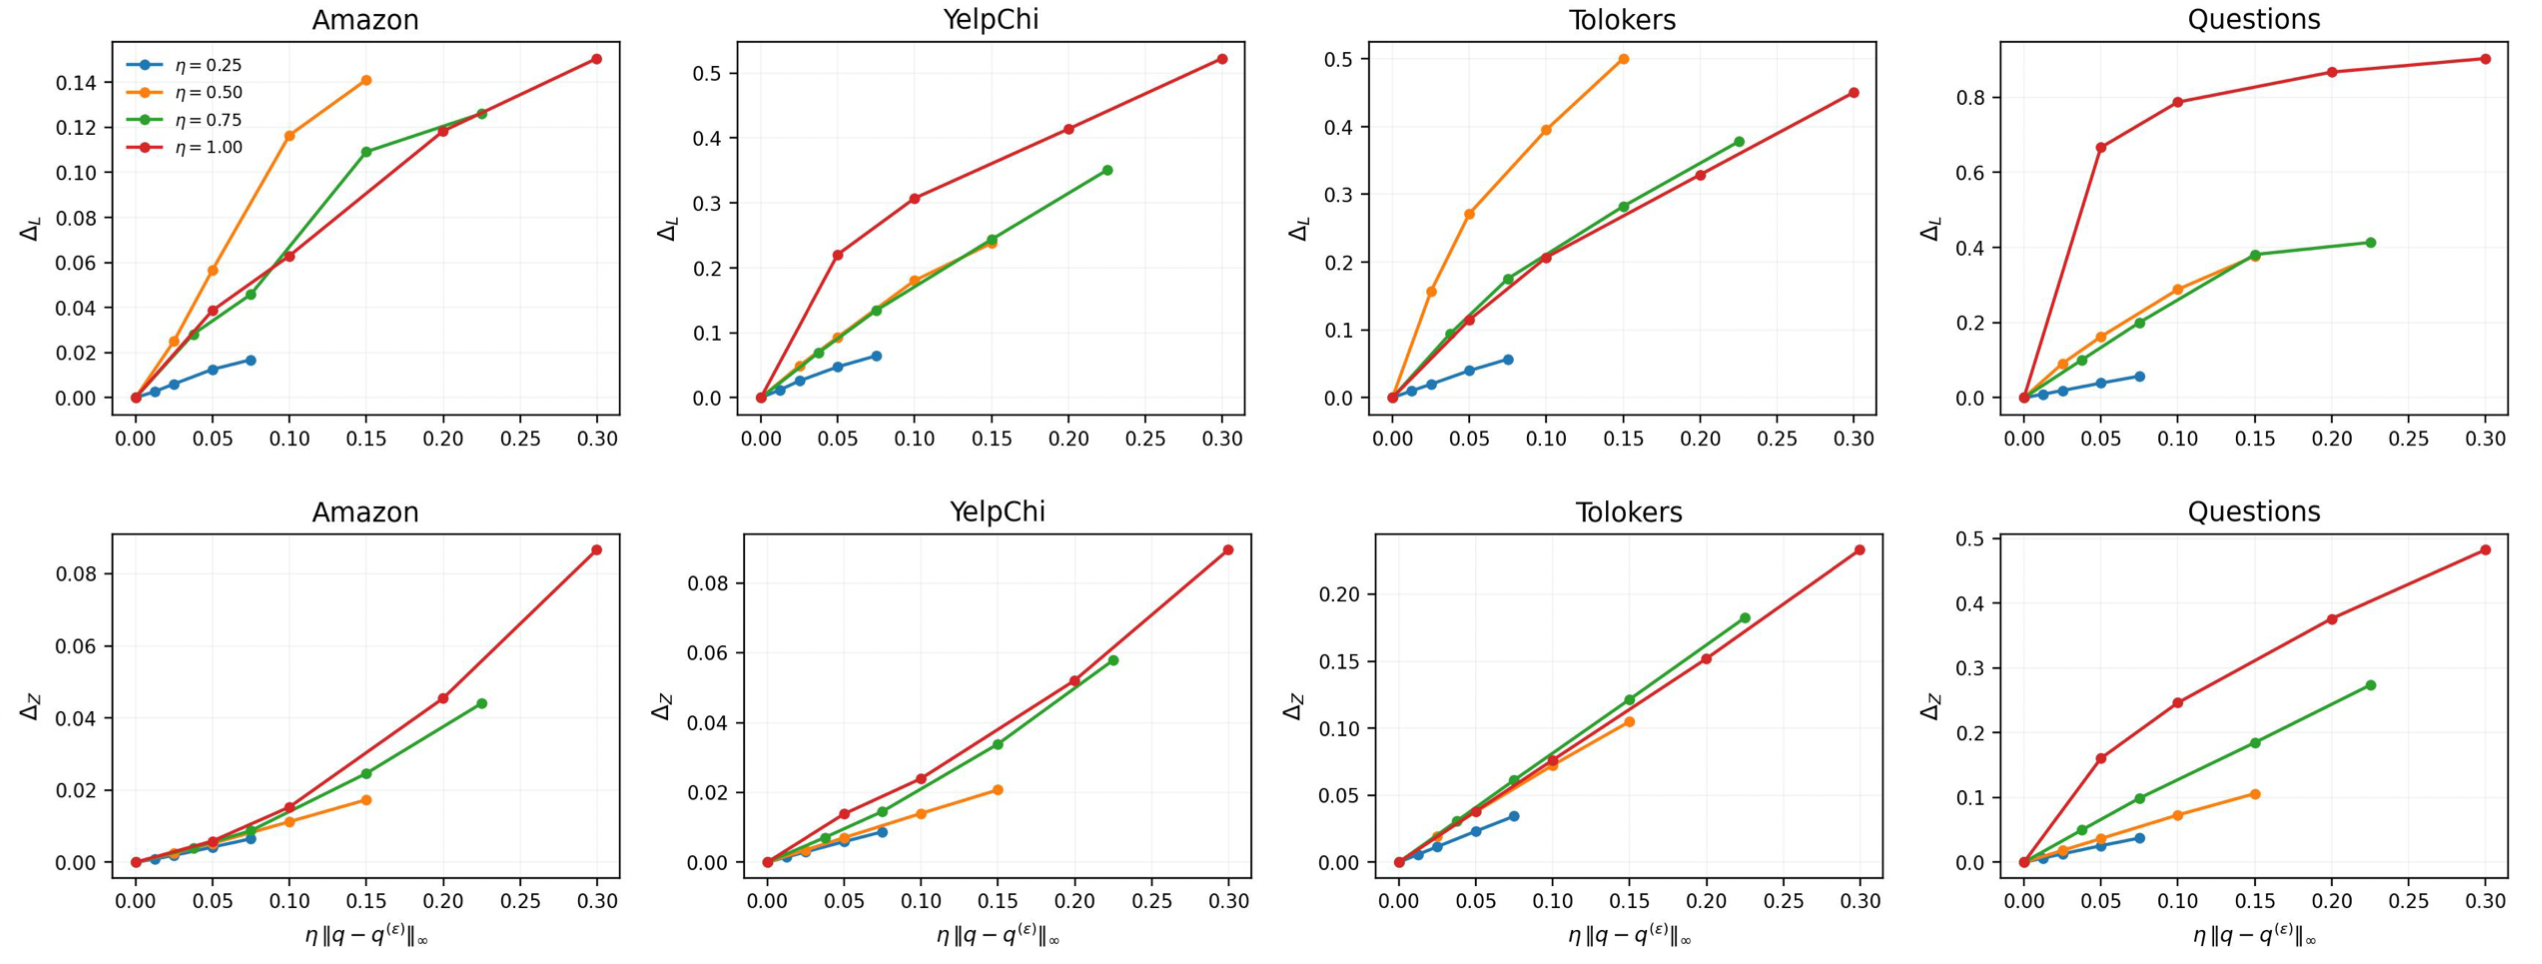
\includegraphics[width=\linewidth]{images/rq3.png}}
\caption{Robustness to edge-calibration errors under different fixed calibration strengths $\eta$.
The horizontal axis denotes the scaled calibration perturbation $\eta\|q-q^{(\epsilon)}\|_\infty$.
The top row plots the operator perturbation $\Delta_L=\|L_\eta(q)-L_\eta(q^{(\epsilon)})\|_2$ and the bottom row plots the normalized representation perturbation $\Delta_Z=\|Z(q)-Z(q^{(\epsilon)})\|_F/\|H^{(0)}\|_F$, averaged over 10 splits.} 
\label{fig:rq3}
% \vspace{-10pt}
\end{figure*}

We analyze the empirical implications of Theorems~\ref{thm:stab} and~\ref{thm:repr} by perturbing the frozen edge-calibration scores $\hat{q}_{uv}$ and its calibration strength while keeping the later training pipeline the same.
First, the learned $\hat{q}$ is kept as the fixed $q$. We then add a small error $\epsilon$ to get a perturbation of $q$, denoted as $q^{(\epsilon)}$.
Specifically, we generate $q^{(\epsilon)}=\mathrm{clip}(q+\Delta_\epsilon,0,1)$ with $\Delta_\epsilon\sim U(-\epsilon,\epsilon)$ drawn i.i.d.\ per non-self-loop edge and vary $\epsilon\in\{0,0.05,0.10,0.20,0.30\}$.
Then, the approximation errors are computed as $\Delta_q=\|q-q^{(\epsilon)}\|_\infty$ after clipping.
We also fix $\eta\in\{0.25,0.50,0.75,1.00\}$. 
Since $\eta$ is fixed within each experiment, the calibration strength mismatch term in Theorem~\ref{thm:stab} vanishes, leaving the operator perturbation controlled by the scaled local calibration error $\eta\,\eloc(q,q^{(\epsilon)})$, which is at most the scaled worst-edge error $\eta\|q-q^{(\epsilon)}\|_\infty$ on the horizontal axis.
This error is also considered in the subsequent robustness analysis of the mapping function $\bm Z$ in Theorem~\ref{thm:repr}.
The plots of the perturbation effects are presented in Fig.~\ref{fig:rq3}.

Figure~\ref{fig:rq3} shows that $\Delta_L$ systematically increases as this quantity grows across all four datasets, with weak calibration remaining in a substantially lower-perturbation regime. 
The curves are not expected to share a common slope, since the theorem gives a perturbation bound rather than an equality and the realized sensitivity also depends on graph normalization and topology. 
Nevertheless, the observed scaling highlights that $\eta$ directly modulates how calibration uncertainty enters the signed propagation operator, which is consistent with the central claim of Theorem~\ref{thm:stab}.

The second row of Fig.~\ref{fig:rq3} further shows that perturbations of the signed operator propagate to the learned spectral representation.
$\Delta_Z$ generally increases with the induced operator error, while remaining markedly smaller than $\Delta_L$ in several settings. 
This behavior indicates that the multi-channel spectral transformation does not amplify the errors from edge-calibration phase, which is highlighted by the vanishing of the gate $\bm g$ in the bound of Theorem~\ref{thm:repr}.
Importantly, these results sharpen the role of soft signing in ESO-GAD. 
The calibration strength $\eta$ is not only a parameter controlling the amount of heterophilic information injected into propagation.
It also provides an explicit robustness mechanism that regulates exposure to errors in the edge-heterophily estimator.
%Thus, ESO-GAD couples edge-semantic exploitation with controlled sensitivity to calibration uncertainty, providing a principled alternative to committing fully to noisy heterophilic estimates.
%Figure~\ref{fig:rq3} therefore offers empirical evidence for the structural perturbation pathway underlying Theorem~1, rather than claiming exact tightness of the theoretical bounds or a universal relationship with downstream accuracy.

\subsubsection{Analysis on KL-regularized spectral gating}
\label{sec:rq6}
In the aggregation gate of Eq.~\eqref{eq:gate}, 
we compare the full ESO-GAD gate with two simplified alternatives: fixed uniform aggregation and learnable aggregation without KL regularization. 
Results are averaged over the same 10 random splits.
As shown in Table~\ref{tab:rq6-main}, Learnable+KL achieves the best AUPRC and AUROC on Amazon, YelpChi, and Questions, while remaining competitive on Tolokers. 
These results indicate that adaptive spectral aggregation is generally preferable to uniform weighting, with KL regularization providing additional benefit over unconstrained gating on most datasets.
%The results further support the role of KL regularization in the coupled optimization of the spectral gate and the learnable signed operator $L_\eta$. 
%While the learnable gate enables dataset-adaptive spectral weighting, the KL term discourages premature concentration on a small subset of channels as $L_\eta$ evolves during training. 
%The small exception on Tolokers suggests that KL regularization is not uniformly beneficial, but rather provides a more robust trade-off between spectral adaptivity and regularization. 
%Overall, the results support KL-regularized learnable gating as an effective balance between spectral adaptivity and stable channel utilization in ESO-GAD.

\begin{table*}[t]
\centering
\caption{Comparison between different aggregator gate choices to produce the representation $\bm Z$ from different filter bands. %The results are reported on 4 datasets over 10 runs with AUPRC and AUROC metrics.
}
\label{tab:rq6-main}
\resizebox{0.85\textwidth}{!}{
\begin{tabular}{lcccccccc}
\hline
& \multicolumn{2}{c}{\textbf{Amazon}}
& \multicolumn{2}{c}{\textbf{YelpChi}}
& \multicolumn{2}{c}{\textbf{Tolokers}}
& \multicolumn{2}{c}{\textbf{Questions}} \\
\textbf{Variant}
& \textbf{AUPRC} & \textbf{AUROC}
& \textbf{AUPRC} & \textbf{AUROC}
& \textbf{AUPRC} & \textbf{AUROC}
& \textbf{AUPRC} & \textbf{AUROC} \\
\hline

Uniform Gate
& 82.80$_{\pm2.11}$
& 93.04$_{\pm1.74}$
& 27.90$_{\pm3.38}$
& 68.58$_{\pm4.32}$
& \underline{40.31}$_{\pm2.41}$
& 73.05$_{\pm1.59}$
& \underline{9.25}$_{\pm1.82}$
& 67.92$_{\pm3.81}$ \\

Learnable, no KL
& \underline{83.06}$_{\pm2.30}$
& \underline{93.68}$_{\pm1.90}$
& \underline{28.17}$_{\pm3.25}$
& \underline{69.14}$_{\pm3.89}$
& \textbf{40.45}$_{\pm2.04}$
& \textbf{73.36}$_{\pm2.20}$
& 9.07$_{\pm1.79}$
& \underline{68.01}$_{\pm3.55}$ \\

Learnable + KL (ESO-GAD)
& \textbf{83.73}$_{\pm1.33}$
& \textbf{94.12}$_{\pm1.37}$
& \textbf{28.87}$_{\pm2.07}$
& \textbf{69.74}$_{\pm2.45}$
& 40.37$_{\pm1.69}$
& \underline{73.18}$_{\pm1.53}$
& \textbf{9.78}$_{\pm1.83}$
& \textbf{68.54}$_{\pm2.55}$ \\

\hline
\end{tabular}
}
\end{table*}

% In the preamble

\subsubsection{Calibration Strength Sensitivity}
We study the impact of the calibration strength $\eta$ on the performance of ESO-GAD by evaluating $\eta\in\{0.25,0.50,0.75,1.00\}$ and adaptive $\eta$ while keeping all other settings fixed.
Figure~\ref{fig:eta-sensitivity} shows that both Amazon and YelpChi favor a moderate strength, with the highest fixed AUPRC among the evaluated values attained at $\eta=0.75$.
Performance does not improve at the reweighting boundary ($\eta=0.5$) but increases for $\eta>0.5$.
Performance subsequently decreases at $\eta=1.0$ on both datasets, suggesting that the estimation errors from the edge calibrator should be controlled properly.
The learned adaptive values also fall near the empirically favorable region, providing evidence that adaptive $\eta$ can recover a competitive calibration value without explicit manual tuning.


\begin{figure}[t]
    \centering
    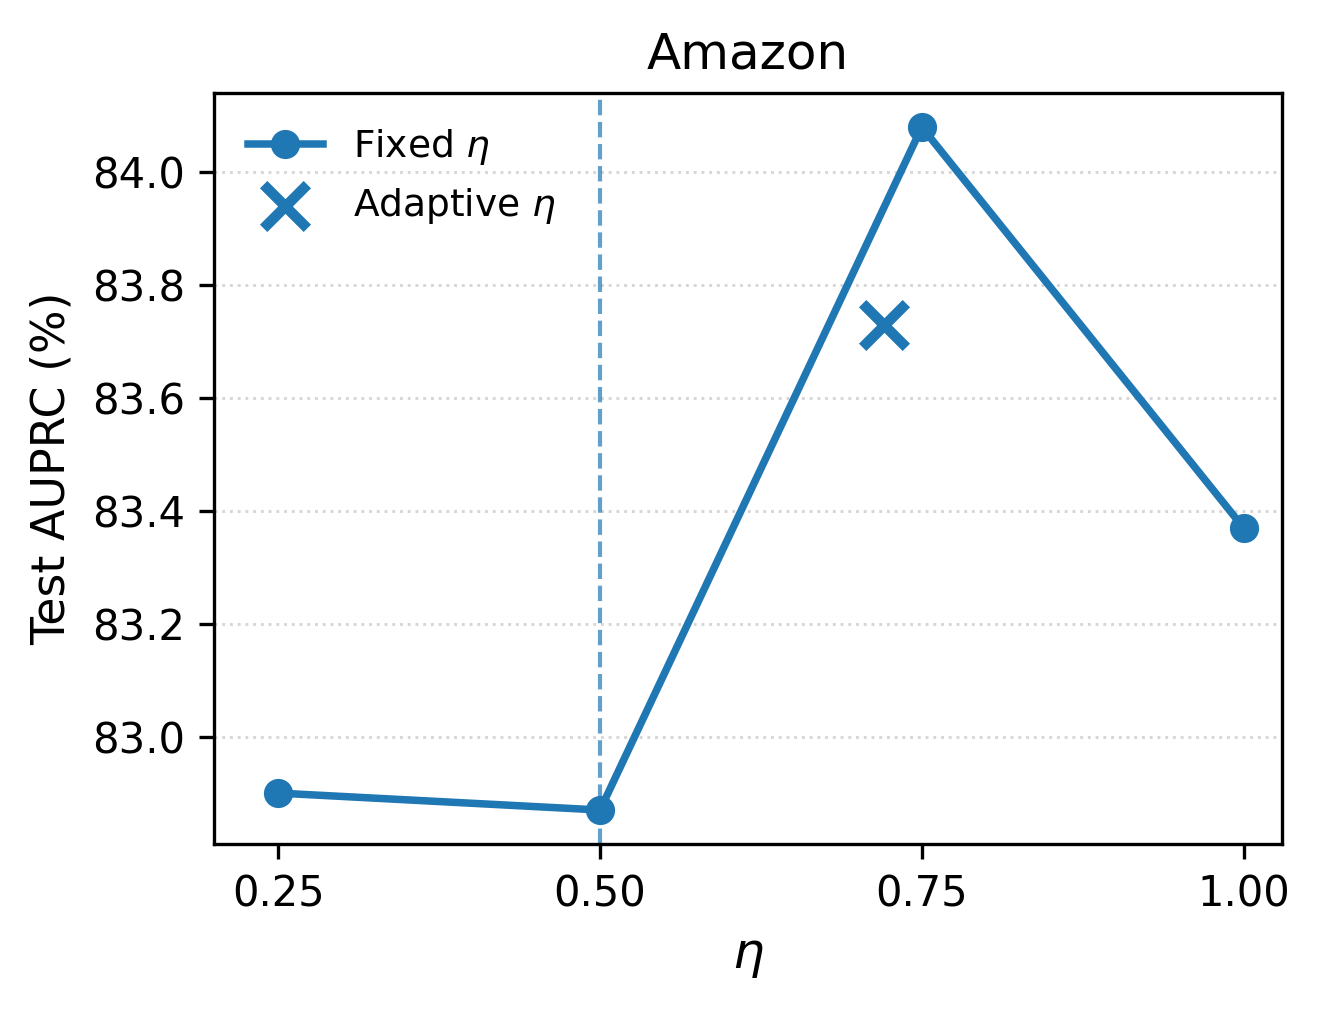
\includegraphics[width=0.48\linewidth]{images/eta_sensitivity_amazon_xlabel_eta.png}
    \hfill
    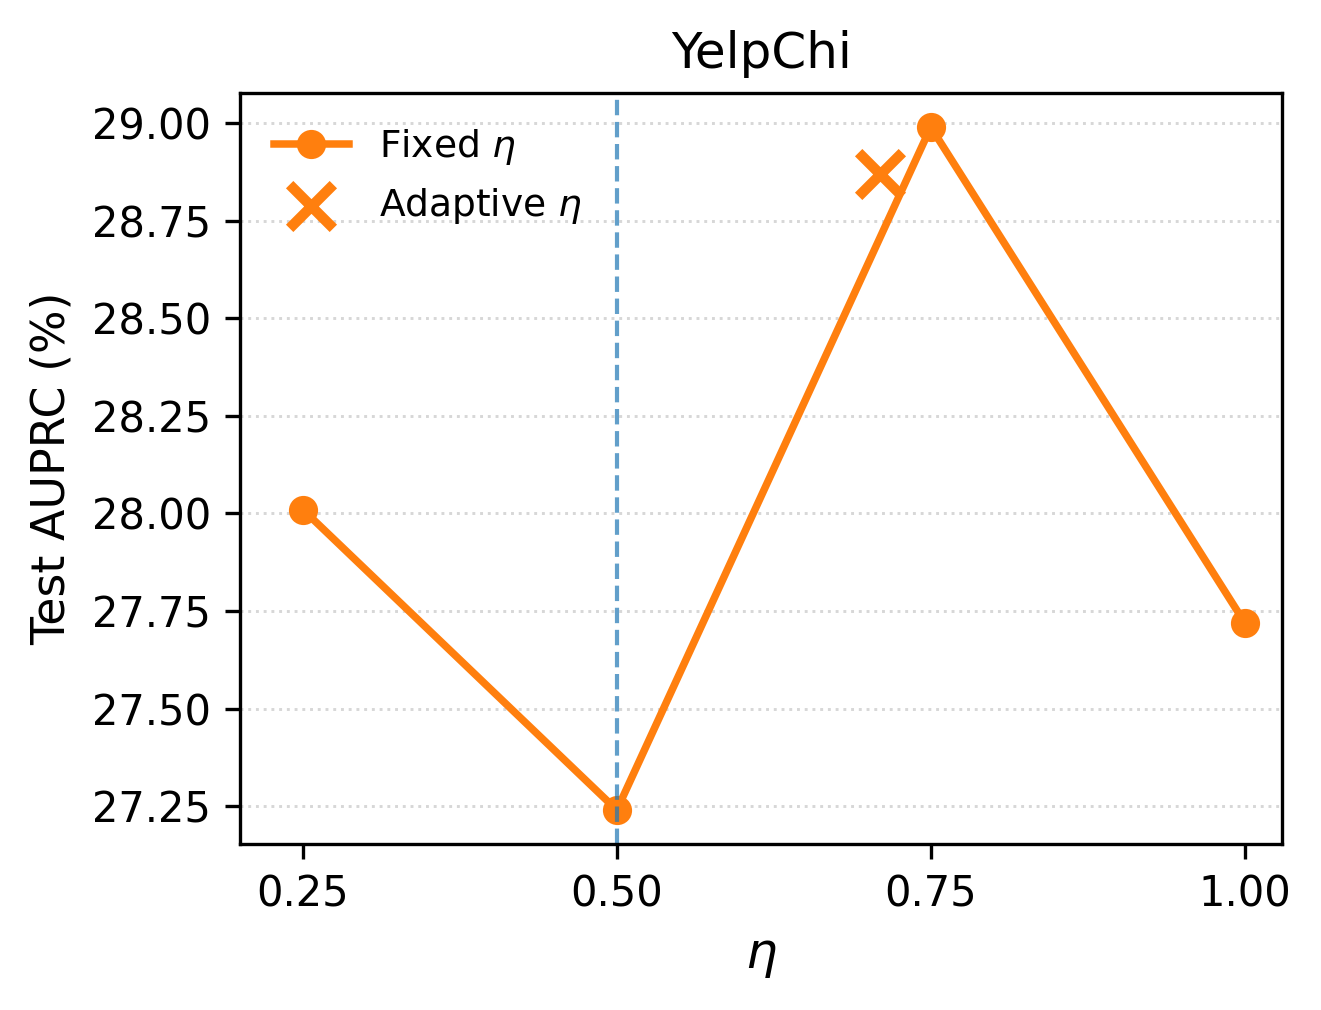
\includegraphics[width=0.48\linewidth]{images/eta_sensitivity_yelpchi_xlabel_eta.png}
    
    \caption{
    Sensitivity to the {calibration strength} $\eta$ on Amazon  and
    YelpChi.
    The line reports test AUPRC under fixed $\eta$, while $\times$ indicates the learned adaptive $\eta$ after the model converges.
    }
    \label{fig:eta-sensitivity}
\end{figure}

\subsubsection{Runtime Analysis}
We compare the training time of ESO-GAD with several spectral methods on a single RTX 3090.
All methods are re-run in the same settings as in Table~\ref{tab:ESO_gad_auroc}.
Reported values are mean end-to-end  training time with 10 runs. For ESO-GAD, we separately report the edge-calibration cost (Phase 1) and signed spectral training cost (Phase 2).

As shown on Table \ref{tab:runtime}, runtime increases with graph size, with all methods remaining lightweight on YelpChi and Amazon but becoming more expensive on T-Finance.
ESO-GAD incurs a clear overhead over BWGNN due to its additional calibration and signed-training stages.
%requiring 7.5/9.9/63.5 s on YelpChi/Amazon/T-Finance, respectively.
In Phase 2, ESO-GAD has to rebuild the operator in Eq.~\eqref{eq:laplacian} after each update of $\eta$, which makes the training time increase in comparison to other spectral baselines.
Nevertheless, this is the trade-off of using an adaptive calibration strength rather than a fixed value.
\begin{table}[t]
\centering
\caption{Mean total training time (s) over 10 seeds.
ESO-GAD is reported with both Phase~1{+}Phase~2 (P1+P2).}
\label{tab:runtime}
\resizebox{\columnwidth}{!}{%
\begin{tabular}{lrrrr}
\hline
Dataset & BWGNN & GHRN & ChiGAD & ESO-GAD $(P1+P2)$ \\
\hline
YelpChi   & 1.2 & 1.3 & 2.6  & 3.2{+}4.2 \ (7.5) \\
Amazon     & 1.0 & 1.4 & 2.5  & 4.4{+}5.6 \ (9.9) \\
T-Finance & 8.2 & 9.8 & 14.8 & 29.7{+}33.7 \ (63.5) \\
\hline
\end{tabular}}
\end{table}

